%\documentclass[11pt]{article}
\documentclass[answers]{exam}

\usepackage{amsmath}
%\usepackage{extsizes}
\usepackage{amsmath,amssymb}
%\usepackage{omegavn,ocmrvn}
%\usepackage[utf8x]{inputenc}
\usepackage[utf8]{vietnam}
\DeclareUnicodeCharacter{00A0}{ }

\usepackage{listings}
\lstset{language=Python}          % Set your language (you can change the language for each code-block optionally)

\usepackage{longtable}
\usepackage{answers}
\usepackage{graphicx}
\usepackage{array}
\usepackage{pifont}
\usepackage{picinpar}
\usepackage{enumerate}
\usepackage[top=3.0cm, bottom=3.5cm, left=3.5cm, right=2.5cm] {geometry}
\usepackage{hyperref}


\newtheorem{bt}{Câu}
\newcommand{\RR}{\mathbb R}
\Newassociation{sol}{Solution}{ans}
\newtheorem{ex}{Câu}
\renewcommand{\solutionstyle}[1]{\textbf{ #1}.}


\begin{document}
% \noindent
\begin{tabular*}
	{\linewidth}{c>{\centering\hspace{0pt}} p{.7\textwidth}}
	Trường ĐHKHTN, ĐHQGHN & {\bf Học Kỳ 1 (2021-2022)}
	\tabularnewline
	{K64 TTƯD - Lớp thầy Hà Phi} & {\bf Bài Tập Giải Tích Số. No 1 \\ \today}
	\tabularnewline
	\rule{1in}{1pt}  \small  & \rule{2in}{1pt} %(Due date:)
	\tabularnewline
	
	%  \tabularnewline
	%  &(Đề thi có 1 trang)
\end{tabular*}
%
%\Opensolutionfile{ans}[ans1]
\printanswers

\centering{BÀI TẬP THỰC HÀNH TRÊN LỚP}

\begin{bt}
	Khai triển Maclaurin của hàm $arctan$ là $x - (1/3)x^3 + (1/5)x^5 + \mathcal{O}(x^7)$. Hãy tính sai số tuyệt đối và sai số tương đối của $\pi$ bằng cách sử dụng đa thức đó để xấp xỉ hàm $arctan$ đến 6 chữ số thập phân trong các biểu thức sau. Viết script để tính toán trong Python.
	%
	\begin{equation*} 
		a.\ 4 \ (\arctan \frac{1}{2} + arctan \frac{1}{3}) \hskip 2cm b.\ 16 \ arctan \frac{1}{5} - 4 \ arctan \frac{1}{239}.
	\end{equation*}
	%
\end{bt}

\begin{bt} \textbf{Cải tiến việc giải số phương trình bậc hai} \ Xét phương trình bậc hai $ax^2 + bx+c = 0$ và giả sử rằng $a\not= 0$ và $\Delta : b^2-4ac>0$. Các nghiệm của phương trình bậc hai là
	%
	\[
	x_{1,2} =  \dfrac{-b \pm \sqrt{\Delta}}{2a}
	\]
	% 
	a) Em có nhận xét gì trong trường hợp $|b| \approx \sqrt{\Delta}$. \\
	b) Áp dụng để tìm nghiệm của các phương trình sau
	\begin{enumerate}
		\item[i)] $x^2 - 10,000.0001 x + 1 = 0$, 
		\item[ii)] $x^2 - 10,000,000.000001 x + 1 = 0$.
	\end{enumerate}
	c) Hãy viết một hàm số trong Python để giải gần đúng phương trình bậc hai ở trên.
\end{bt}

\begin{bt} 
Một Hacker đã viết nên 1 chương trình để hack các giao dịch của một ngân hàng và gửi chúng vào tài khoản của chính anh ta. Trong bài tập này, các em sẽ mô phỏng chương trình để xác định mất bao lâu để trở thành tỷ phú theo cách này.
Giả sử rằng các em có quyền truy cập vào 50.000 tài khoản ngân hàng. Ban đầu, các em có thể coi số dư tài khoản là một con số ngẫu nhiên giữa 1 triệu VND và 100 triệu VND (thực ra điều này không quá quan trọng). Lãi suất hàng năm trên các tài khoản là $5\%$ và tiền lãi được cộng dồn hàng ngày và được cộng vào các tài khoản, ngoại trừ các con số lẻ của ngàn đồng sẽ bị cắt bớt (ví dụ 3532.42 VND sẽ bị cắt thành 3000 VND). Số tiền này sẽ được gửi vào một tài khoản hacker có số dư ban đầu là $0$ VND. \\

Hãy viết chương trình PYTHON mô phỏng kịch bản trên. Các em có thể thiết lập các tài khoản ban đầu bằng các lệnh 
%
\begin{lstlisting}[frame=single] 
from numpy.random import rand

a = 1e+6    # so tien toi thieu
b = 1e+9    # so tien toi da
n = 50000   # 50.000 tai khoan

# Tao so tien trong moi tai khoan 1 cach ngau nhien trong pham vi a, b
tai_khoan = a + (b-a) * rand(n,1)
\end{lstlisting}
%
Chú ý cần viết chương trình PYTHON để tăng các tài khoản lên (5/365)\% tiền lãi mỗi ngày, đặt số tiền đã cắt bớt vào một tài khoản, các em sẽ gọi là $tai\_khoan\_hacker$. Giả sử rằng tài khoản hacker có thể giữ số tiền nhỏ (nghĩa là không cắt bớt giá trị của tài khoản này) và để tài khoản hacker cũng tích lũy lãi suất hàng ngày. Chạy code của các em để xác định mất bao nhiêu ngày để các em trở thành tỷ phú.
\end{bt}

\begin{bt}
Trong Chiến tranh vùng Vịnh năm 1991, hệ thống phòng thủ tên lửa Patriot đã thất bại do lỗi bay vòng. Rắc rối bắt nguồn từ một máy tính thực hiện các phép tính theo dõi với đồng hồ bên trong có giá trị số nguyên với đơn vị là một phần mười giây, được chuyển đổi thành giây bằng cách nhân với xấp xỉ nhị phân 24 bit (như Hình \ref{fig:onetenthbinary}) với mười: \\
%
\begin{figure}[!h]
	\centering
	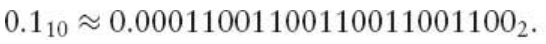
\includegraphics[width=0.5\linewidth]{One_tenth_binary}
	\caption{Biểu diễn nhị phân của 1/10 giây trong máy tính của hệ thống phòng thủ tên lửa Patriot}
	\label{fig:onetenthbinary}
\end{figure}
%
(a) Chuyển đổi số nhị phân trong công thức trên thành phân số. Gọi nó là x. \\
(b) Sai số tuyệt đối của x so với $1/10$ là bao nhiêu? \\
(c) Sai số thời gian tính bằng giây sau 100 giờ hoạt động là bao nhiêu? \\
(d) Trong chiến tranh năm 1991, một tên lửa Scud đã di chuyển với vận tốc xấp xỉ Mach 5 (1676,4 mét/giây). Tìm khoảng cách mà tên lửa Scud sẽ di chuyển trong thời gian sai số được tính trong (c).
\textbf{Vào ngày 25 tháng 2 năm 1991, một hệ thống pin Patriot, để bảo vệ Căn cứ Không quân Dhahran, đã hoạt động hơn 100 giờ liên tục. Lỗi vòng quay khiến hệ thống không theo dõi được tên lửa Scud đang bay tới, tên lửa này đã trượt qua hệ thống phòng thủ và phát nổ trong doanh trại quân đội Hoa Kỳ, giết chết 28 lính Mỹ.} 
\end{bt}

\vskip .5cm

\centerline{——————————— Bài Tập Tự Luyện ——————————}

\begin{bt}	Ôn tập về chữ số chắc, đánh mất các chữ số chắc và một số cách khắc phục. \\
	\begin{tabular}{ll}
		i) $\ln(x+1)-\ln(x)$ với $x$ rất rất lớn, \qquad	&  iv) $\sqrt{x+1} - \sqrt{1-x}$ với $x\approx 0$, \\
		ii) $\cos^2(x) - \sin^2(x)$ với $x\approx \dfrac{\pi}{4}$, \qquad	&  v) $\ln(x) - 1$ với $x \approx e$, \\
		iii) $f(x)=\sqrt{x^2+1}-x$ với $x$ rất rất lớn,	\qquad & vi) $f(x)= \sqrt{ \dfrac{1+\cos(x)}{2}}$ tại $x\approx \pi$. \\
	\end{tabular}
\end{bt}

\begin{bt}
Nếu dùng chuỗi Maclaurin để xấp xỉ $\sin(1)$ với sai số tuyệt đối nhỏ hơn $5 * 10^{-7}$ thì cần bao nhiêu số hạng. Viết script trong Python để tìm số số hạng cần thiết và tính xấp xỉ, sai số tuyệt đối và tương đối của xấp xỉ đó.
\end{bt}

\begin{bt} 
Hãy viết script tính toán $\ln(1.2)$ tới chính xác 7 chữ số thập phân sử dụng khai triển 
%
\[
\ln \dfrac{1+x}{1-x} = 2 \left( x + \dfrac{x^3}{3} + \dfrac{x^5}{5} + \dfrac{x^7}{7} + ...  \right)
\]
%
\end{bt}

\begin{bt}
Hãy sử dụng đa thức Taylor bậc $9$ của hàm $e^x$ và phép cắt 5 chữ số sau dấu chấm thập phân để xấp xỉ $e^{-5}$ bằng các xấp xỉ sau.
%
\[
a.\ e^{-5} \approx \sum_{n=0}^{9}((-5)^n/n!) \qquad \qquad \qquad b.\ e^{-5} = \frac{1}{e^5} \approx \frac{1}{\sum_{n=0}^{9}(5^n/n!)}. 
\]
%
Công thức nào trong 2 công thức (a) và (b) cho ta giá trị xấp xỉ tốt hơn, vì sao?
\end{bt}

\centerline{———————————Hết——————————}

%\vspace{1cm}
%\noindent{\bf Chú ý:} {\it Cán bộ coi thi không giải thích gì thêm}\\
%\vspace{0.4cm}
%\noindent{\bf Họ và tên học sinh: \rule{3in}{.01pt} Lớp: \hrulefill}
%\Closesolutionfile{ans}
%\newpage
%\begin{center}
%{\LARGE{\bf ĐÁP ÁN}}
%\end{center}
%\begin{Solution}{1}
	\begin{figure}[h!]
		\centering
		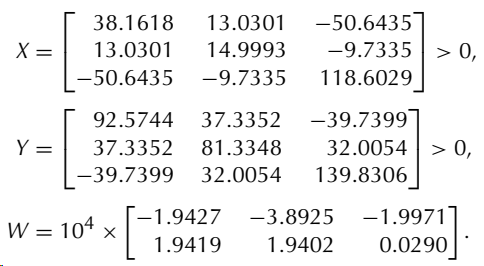
\includegraphics[width=0.7\linewidth]{Solution1/screenshot001}
		\caption[Exercise 1.2.5, Burden-Faires, 8ed.]{}
		\caption{}
		\label{fig:screenshot001}
	\end{figure}
\end{Solution}
 
   
\end{document}